\section{Justificación}
La República Mexicana se encuentra en una de las regiones sísmicas más activas del mundo, conocida como el Cinturón Circumpacífico ~\cite{SGM2023}. Esta alta actividad sísmica se debe a la interacción de varias placas tectónicas, incluyendo Norteamérica, Cocos, Pacífico, Rivera y Caribe como se puede observar en la figura \ref{fig:Mapa de placas tectonicas}~\cite{SGM}, así como a fallas locales en varios estados. Los estados más afectados son Chiapas, Guerrero, Oaxaca, Michoacán, Colima y Jalisco, debido a la interacción de las placas oceánicas de Cocos y Rivera con Norteamérica y el Caribe en la costa del Pacífico. 
\begin{figure}[H]
    \centering
    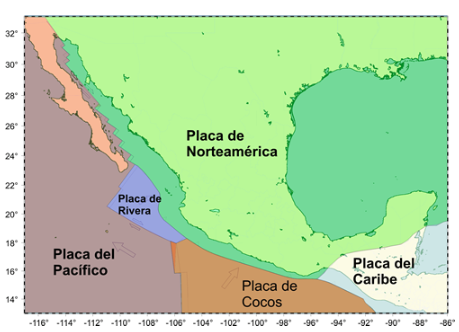
\includegraphics[width=0.75\textwidth]{img/placas.png}
    \caption{Placas tectónicas.}
    \label{fig:Mapa de placas tectonicas}
\end{figure}

 
Aunque los epicentros se localizan en diversos puntos del Pacífico, la Ciudad de México, aunque no está en la costa, se ve afectada debido a su proximidad y a la naturaleza de su terreno. El estudio de la actividad sísmica en México comenzó a principios del siglo XX, y se inauguró la red sismológica mexicana en 1910. Actualmente, el Servicio Sismológico Nacional \cite{SSN} opera una red de 35 estaciones sismológicas y reporta en promedio la ocurrencia de 4 sismos por día de magnitud M > 3.0. Además del SSN, existen otros grupos de investigación como el CICESE y la RESNOR que estudian la actividad sísmica en el Golfo de California y la falla de San Andrés, respectivamente. También hay instituciones educativas que realizan estudios de sismicidad regional y mantienen comunicación para compartir avances\cite{SGM2023}.

En el año 2022, la sismicidad en México continuó siendo una preocupación importante, ya que se registraron varios sismos de magnitud considerable~\cite{SSN} ver figura \ref{fig:Mapa de sismisidad anual 2022}. Se puede observar que algunos de estos eventos sísmicos alcanzaron magnitudes superiores a 6.0, lo que demuestra la necesidad de contar con un sistema eficiente para monitorear y analizar la actividad sísmica en la región. La distribución de estos eventos a lo largo del año también muestra que la actividad sísmica en México no se limita a un período específico, sino que se presenta a lo largo de todo el año, lo que refuerza la importancia de contar con un sistema de monitoreo y análisis en tiempo real.
\begin{figure}[H]
    \centering
    \includegraphics[width=0.75\textwidth]{img/SSNMX_mapa_sismicidad_2022_web.png}
    \caption{Mapa de sismisidad anual 2022}
    \label{fig:Mapa de sismisidad anual 2022}
\end{figure}


Actualmente se tiene la necesidad de desarrollar un sistema unificado de recopilación y procesamiento de los datos asociados a posibles precursores sísmicos provenientes de diversas fuentes, como estaciones de monitoreo, catálogos sísmicos como el del servicio sismológico de México, etc. Aunado a la limitada disponibilidad de datos, los sistemas actuales no tratan ni analizan de manera sistemática los datos recolectados, lo que dificulta la comprensión de los precursores sísmicos y la toma de decisiones informadas para la reducción y gestión del riesgo de desastres.

Este proyecto busca abordar esta brecha mediante el análisis ya conocido de los posibles precursores sísmicos utilizando los datos disponibles ~\cite{mcnally1983seismic}~\cite{scholz1997whatever}~\cite{varotsos1984physical}~\cite{yepez1995electric}~\cite{hayakawa1999fractal}~\cite{hayakawa2007monitoring}~\cite{Bhardwaj2021}. A través de este análisis, se pretende mejorar nuestra comprensión de los fenomenos que preceden a los sismos y establecer patrones de comportamiento relevantes de dichos precursores para evaluar la actividad sísmica en un período de tiempo específico\cite{Bhardwaj2021}. Al fortalecer nuestra capacidad para analizar y monitorear estos precursores, el sistema propuesto contribuirá a respaldar la toma de decisiones informadas en la gestión del riesgo sísmico. Esto podría tener un impacto significativo en la prevención y mitigación de los efectos adversos de los sismos en la población y la infraestructura.